\documentclass[tikz,border=8pt]{standalone}
% Shared look for every TikZ diagram. Load with \input{../../tools/tikz-style.tex}
\usepackage[T1]{fontenc}
\usepackage{lmodern}
\renewcommand{\sfdefault}{lmr}  % diagrams use the same serif as the text
\usetikzlibrary{arrows.meta, positioning, shapes.geometric, calc, fit, backgrounds}
\definecolor{cblue}{HTML}{4C78A8}
\definecolor{corange}{HTML}{F58518}
\definecolor{cgreen}{HTML}{54A24B}
\definecolor{cred}{HTML}{E45756}
\definecolor{cpurple}{HTML}{B279A2}
\definecolor{cgrey}{HTML}{6B6B6B}
\tikzset{
  every picture/.style={font=\sffamily, line width=1.2pt},
  box/.style={draw=#1, fill=#1!12, rounded corners=4pt, align=center, inner sep=7pt, minimum height=1.1cm},
  box/.default=cgrey,
  arrow/.style={-{Stealth[length=3mm]}, draw=cgrey, line width=1.4pt},
  title/.style={font=\sffamily\bfseries\Large},
  note/.style={font=\sffamily\small, text=cgrey, align=center},
}
\AtBeginDocument{\hyphenpenalty=10000 \exhyphenpenalty=10000}

\begin{document}
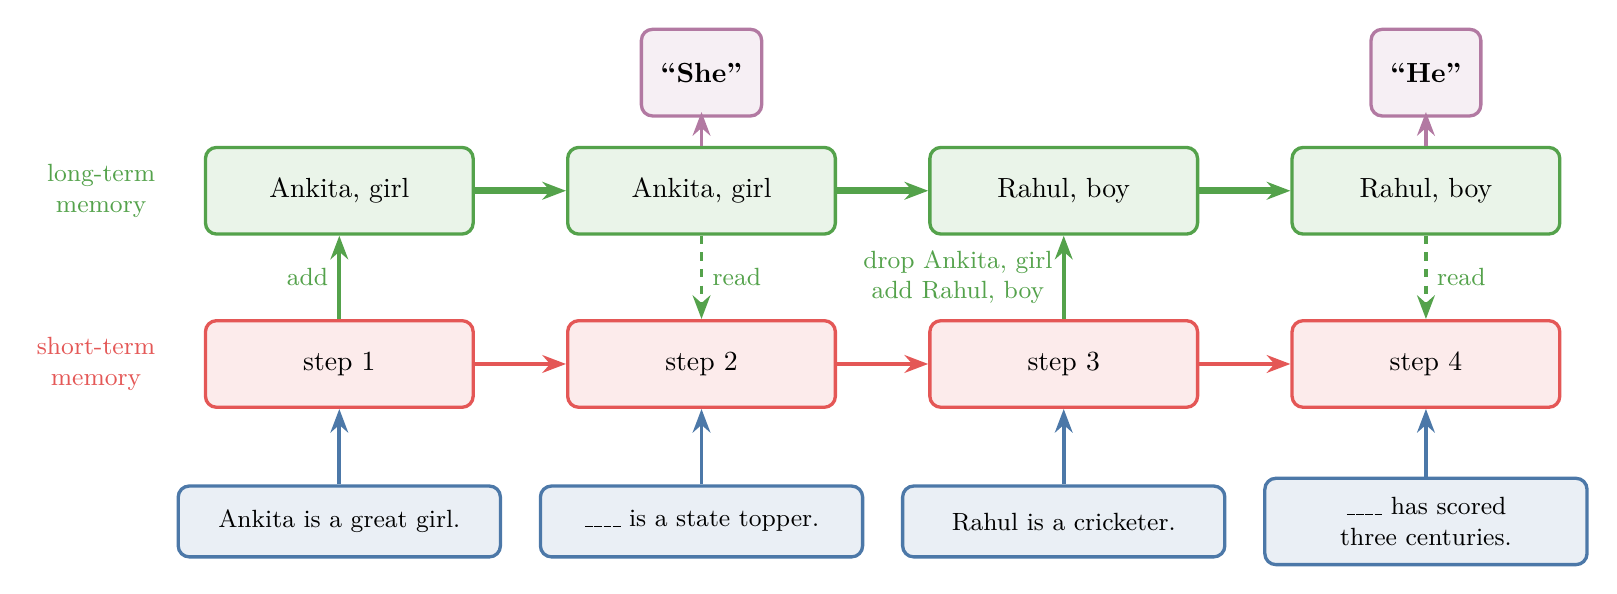
\begin{tikzpicture}[lt/.style={box=cgreen, minimum width=3.4cm}, st/.style={box=cred, minimum width=3.4cm},
  inp/.style={box=cblue, text width=3.6cm, font=\sffamily\small, minimum height=0.9cm}]
  \node[note, anchor=east, text=cgreen] at (-0.4,2.2) {long-term\\memory};
  \node[note, anchor=east, text=cred] at (-0.4,0) {short-term\\memory};
  \foreach \i/\x/\lab/\long in {1/1.8/{Ankita is a great girl.}/{Ankita, girl}, 2/6.4/{\_\_\_\_ is a state topper.}/{Ankita, girl}, 3/11.0/{Rahul is a cricketer.}/{Rahul, boy}, 4/15.6/{\_\_\_\_ has scored three centuries.}/{Rahul, boy}} {
    \node[lt] (c\i) at (\x,2.2) {\long};
    \node[st] (h\i) at (\x,0) {step \i};
    \node[inp] (x\i) at (\x,-2.0) {\lab};
    \draw[arrow, draw=cblue] (x\i) -- (h\i);
  }
  \foreach \i/\j in {1/2, 2/3, 3/4} { \draw[arrow, draw=cgreen, line width=2.5pt] (c\i) -- (c\j); \draw[arrow, draw=cred] (h\i) -- (h\j); }
  \draw[arrow, draw=cgreen] (h1) -- node[left, note, text=cgreen] {add} (c1);
  \draw[arrow, draw=cgreen] (h3) -- node[left, note, text=cgreen] {drop Ankita, girl\\add Rahul, boy} (c3);
  \draw[arrow, draw=cgreen, dashed] (c2) -- node[right, note, text=cgreen] {read} (h2);
  \draw[arrow, draw=cgreen, dashed] (c4) -- node[right, note, text=cgreen] {read} (h4);
  \node[box=cpurple, font=\sffamily\bfseries] at (6.4,3.7) {``She''};
  \node[box=cpurple, font=\sffamily\bfseries] at (15.6,3.7) {``He''};
  \draw[arrow, draw=cpurple] (c2) -- (6.4,3.2);
  \draw[arrow, draw=cpurple] (c4) -- (15.6,3.2);
\end{tikzpicture}
\end{document}
